% 第 19 题长方体图：按固定源内容流矢量层精确值复刻（1 pt → 0.03515 cm）。
% 原点取顶点 A（源页 (598.6953, 557.6328) pt），y 向上。
% 标准斜二测：前底边 AB 足尺 120.1523 pt（题设 AB=2 → 60.076 pt/单位）；侧棱竖直 60.074；
% 深度方向 45°、长度折半 60.065；全图按题设尺寸精确作画（E、F 为棱中点，实测差 ≤0.003 pt）。
% 实线 12 段：9 条可见棱 + 辅助线 A₁–E、C₁–F 与顶面对角线 A₁–C₁；
% 虚线 5 段：被遮棱 AD、DC、DD₁ 与题设直线 D₁C、平面边 EF（节距照源 [on 2.989 off 2.989]）。
% 全图无点记号、无箭头、无填充；十个标签照源字形包围盒中心定位（显式坐标、inner sep=0）。
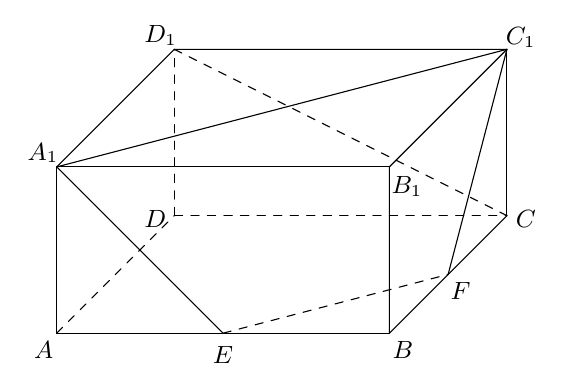
\begin{tikzpicture}[line cap=round,line join=round,font=\small,x=0.03515cm,y=0.03515cm]
% ===== 实线（12 段）=====
\draw[line width=0.398bp] (0,0)--(120.1523,0);   % A–B
\draw[line width=0.398bp] (120.1523,0)--(162.625,42.4726);   % B–C
\draw[line width=0.398bp] (0,60.0742)--(120.1524,60.0742);   % A1–B1
\draw[line width=0.398bp] (120.1524,60.0742)--(162.625,102.5508);   % B1–C1
\draw[line width=0.398bp] (162.625,102.5508)--(42.4727,102.5469);   % C1–D1
\draw[line width=0.398bp] (42.4727,102.5469)--(0,60.0742);   % D1–A1
\draw[line width=0.398bp] (0,0)--(0,60.0742);   % A–A1
\draw[line width=0.398bp] (120.1523,0)--(120.1524,60.0742);   % B–B1
\draw[line width=0.398bp] (162.625,42.4726)--(162.625,102.5508);   % C–C1
\draw[line width=0.398bp] (0,60.0742)--(60.0742,0);   % A1–E
\draw[line width=0.398bp] (162.625,102.5508)--(141.3867,21.2383);   % C1–F
\draw[line width=0.398bp] (0,60.0742)--(162.625,102.5508);   % A1–C1
% ===== 虚线（5 段）=====
\draw[dash pattern=on 2.989pt off 2.989pt, line width=0.398bp] (0,0)--(42.4727,42.4726);   % A–D
\draw[dash pattern=on 2.989pt off 2.989pt, line width=0.398bp] (42.4727,42.4726)--(162.625,42.4726);   % D–C
\draw[dash pattern=on 2.989pt off 2.989pt, line width=0.398bp] (42.4727,42.4726)--(42.4727,102.5469);   % D–D1
\draw[dash pattern=on 2.989pt off 2.989pt, line width=0.398bp] (42.4727,102.5469)--(162.625,42.4726);   % D1–C
\draw[dash pattern=on 2.989pt off 2.989pt, line width=0.398bp] (60.0742,0)--(141.3867,21.2383);   % E–F
% ===== 标注（照源字形包围盒中心，显式坐标；D₁ 上移后加 overlay——
%       其旧位与 C₁ 同高、本就是包围盒顶界之一，加 overlay 后上移不改变图块尺寸，避免整块重排）=====
\node[anchor=center,inner sep=0] at (-4.7053,-6.0022) {\(A\)};
\node[anchor=center,inner sep=0] at (125.0897,-6.0022) {\(B\)};
\node[anchor=center,inner sep=0] at (169.5097,41.4178) {\(C\)};
\node[anchor=center,inner sep=0] at (35.5947,41.4178) {\(D\)};
\node[anchor=center,inner sep=0] at (60.0197,-8.0422) {\(E\)};
\node[anchor=center,inner sep=0] at (145.8697,15.2428) {\(F\)};
\node[anchor=center,inner sep=0] at (-4.9553,65.1028) {\(A_{1}\)};
\node[anchor=center,inner sep=0] at (126.5147,53.0278) {\(B_{1}\)};
\node[anchor=center,inner sep=0] at (167.5947,106.7928) {\(C_{1}\)};
\node[overlay,anchor=center,inner sep=0] at (37.5347,107.5928) {\(D_{1}\)};
\end{tikzpicture}
